\documentclass[12pt]{article}
\linespread{1.05}
%\usepackage{fancyhdr}
%\usepackage{mathptmx}
%\usepackage{sidecap}
\usepackage{amsfonts, amsmath, amsthm, amssymb, graphicx, verbatim}
\usepackage{xcolor}
\usepackage[margin=1.0in]{geometry}
\usepackage{booktabs} % Top and bottom rules for table
\usepackage[font=small,labelfont=bf]{caption} % Required for specifying captions to tables and figures
\usepackage{amsfonts, amsmath, amsthm, amssymb, graphicx, verbatim} % For math fonts, symbols and environments
\usepackage{wrapfig} % Allows wrapping text around tables and figures
\usepackage[colorinlistoftodos,textsize=tiny]{todonotes} % need xargs for below
%\usepackage{accents}
\usepackage[square,sort,comma,numbers]{natbib}
\usepackage{bbm}
\usepackage{thm-restate}
%\usepackage[backend=bibtex, style=footnote-dw]{biblatex}
%\addbibresource{diss.bib}

\usepackage[colorlinks=true,breaklinks=true,bookmarks=true,urlcolor=blue,
citecolor=blue,linkcolor=blue,bookmarksopen=false,draft=false]{hyperref}
\usepackage{url}
\usepackage{float}
\usepackage{enumitem}

\newcommand{\Comments}{1}
\newcommand{\mynote}[2]{\ifnum\Comments=1\textcolor{#1}{#2}\fi}
\newcommand{\mytodo}[2]{\ifnum\Comments=1%
	\todo[linecolor=#1!80!black,backgroundcolor=#1,bordercolor=#1!80!black]{#2}\fi}
\newcommand{\raf}[1]{\mynote{blue}{[RF: #1]}}
\newcommand{\raft}[1]{\mytodo{blue!20!white}{RF: #1}}
\newcommand{\jessie}[1]{\mynote{green!75!black}{[JF: #1]}}
\newcommand{\jessiet}[1]{\mytodo{green!20!white}{JF: #1}}
\newcommand{\btw}[1]{\mytodo{gray!20!white}{\textcolor{gray}{#1}}}
\newcommand{\future}[1]{}%\mytodo{blue!20!white}{\textcolor{gray!50!black}{FUTURE: #1}}}
\ifnum\Comments=1               % fix margins for todonotes
\setlength{\marginparwidth}{1in}
\fi

%\pagestyle{fancy}
%\lhead{Moving to infinite outcomes}
%\rhead{ }


\newcommand{\reals}{\mathbb{R}}
\newcommand{\posreals}{\reals_{>0}}%{\reals_{++}}
\newcommand{\myderiv}[1]{\tfrac{d}{d#1}} % \partial_{#1}
\newcommand{\myrderiv}[1]{\tfrac{\,d^+\!\!}{d#1}} % \partial_{#1}
\newcommand{\dz}{\myderiv{z}}
\newcommand{\dx}{\myderiv{x}}
\newcommand{\dr}{\myderiv{r}}
\newcommand{\du}{\myderiv{u}}
\newcommand{\rdx}{\myrderiv{x}}
\newcommand{\toto}{\rightrightarrows}

%m upper and lower bounds
\newcommand{\mup}{\overline{m}}
\newcommand{\mlow}{\underline{m}}


% alphabetical order, by convention
\newcommand{\A}{\mathcal{A}}
\newcommand{\B}{\mathcal{B}}
\newcommand{\C}{\mathcal{C}}
\newcommand{\E}{\mathbb{E}}
\newcommand{\F}{\mathcal{F}}
\newcommand{\I}{\mathcal{I}}
\renewcommand{\L}{\mathcal{L}}
\renewcommand{\P}{\mathcal{P}}
\newcommand{\R}{\mathcal{R}}
\newcommand{\Y}{\mathcal{Y}}


\newcommand{\inter}[1]{\mathring{#1}}%\mathrm{int}(#1)}
%\newcommand{\expectedv}[3]{\overline{#1}(#2,#3)}
\newcommand{\expectedv}[3]{\E_{Y\sim{#3}} {#1}(#2,Y)}
\newcommand{\simplex}{\Delta_{\Y}}
\newcommand{\cl}{\mathbf{cl}}
\newcommand{\dom}{\mathbf{dom}}
\newcommand{\effdom}{\mathbf{effdom}}
\newcommand{\codim}{\mathbf{codim}}
\newcommand{\epi}{\mathrm{epi}}
\newcommand{\prop}[1]{\mathrm{prop}[#1]}

\DeclareMathOperator*{\argmax}{arg\,max}
\DeclareMathOperator*{\argmin}{arg\,min}
\DeclareMathOperator*{\arginf}{arg\,inf}
\DeclareMathOperator*{\sgn}{sgn}


\newtheorem{definition}{Definition}	 
\newtheorem{proposition}{Proposition}	 
\newtheorem{condition}{Condition}
\newtheorem{theorem}{Theorem}
\newtheorem{corollary}{Corollary}
\newtheorem{conjecture}{Conjecture}
\newtheorem{lemma}{Lemma}

\begin{document}
\begin{center}
{\large\textbf{Generalizing Theorem 2 to infinite outcomes}}
\end{center}

\section{Background and notation}

\begin{definition}[Domain]
	The domain of a function $f:X \to \reals$ is the set $X$ so that $f(x)$ is defined for all $x \in X$. 
\end{definition}

\begin{definition}[Effective Domain]
	The \emph{effective domain} of a {\color{blue} convex} function $f: X \to \bar \reals$ is the set $S \subseteq X = \{x \in X : f(x) < \infty\}$,
\end{definition}

Let $(\Y, \A, p)$ define a ($\sigma$-finite) measure space.
If we are given a loss $f(u,y)$, we want to understand when $\partial \E_p f(\cdot,Y) = \E_p \partial f(\cdot,Y)$. 

\begin{definition}[Expectation of a closed-valued multifunction]
	 $G:\Y \to 2^\reals$ is defined.
	 $\E_p G = \cl(\{\int \nu(y) p(dy) : \nu \in \L^1_d(\A), \nu(y) \in G(y)\,\, a.s.\})$.
\end{definition}

\begin{definition}[$\otimes$, \cite{folland1999real} Page 20]
	Consider the space $X = \reals^d \times \Y$ and $\pi_\alpha:X \to X_\alpha$ the coordinate maps, where $\alpha \in \{1,2\}$.
	If $\A_\alpha$ is a $\sigma$-algebra on $X_\alpha$ for each $\alpha$,the \emph{product $\sigma$-algebra} on $X$ is the $\sigma$-algebra generated by 
		\begin{equation*}
		\{ E_1 \times E_2 : E_\alpha \in \A_\alpha \}~.~
		\end{equation*}
		We denote this $\sigma$-algebra by $\A_1 \otimes \A_2$.
\end{definition}

\subsection{Definitions needed}
\begin{definition}[Measurable multifunction~\cite{aubin2009set} Definition 8.1.1]
	Consider a measurable space $(\Y, \A)$ and set-valued function $H: \Y \to 2^{\reals^{d+1}}$ with closed images.
	
	The multifunction $H:\Y \to 2^{\reals^{d+1}}$ is $\A$-measurable iff for every open $E \subseteq \reals^{d+1}$, we have $H^{-1}(E) = \{y \in \Y: H(y) \cap E \neq \emptyset \} \in \A$.
\end{definition}

\begin{definition}[$\A$-normal convex integrand]
	A function $f : \reals^d \times \Y \to \bar \reals$ is an $\A$-normal convex integrand if the map
	\begin{equation}
	H^f : y \mapsto \epi(f(\cdot, y))  = \{(u, \alpha) \in \reals^{d+1} : \alpha \geq f(u,y)\}
	\end{equation}
	is a closed convex-valued measurable multifunction.
\end{definition}
Note: the above map is closed if and only if $H^f$ is lower semi-continuous (in $y$), and is convex-valued as $f(\cdot,y)$ is convex in $\reals^d$ for all $y \in \Y$.

%\jessie{Think on how to show this for any expected loss; show true if ??? (e.g. $f$ continuous in $y$)}
\jessie{See who has used this result?}

\begin{definition}[$\A$ convex normal integrand via \cite{castaing2006convex} Definition VII.1]
	A mapping $f : \reals^d \times\Y \to \reals$ is called \emph{normal integrand} if for every fixed $y \in \Y$, we have $f(\cdot, y)$ is lower semi-continuous and $f$ is $\B(\reals^d) \otimes \A$-measurable.
	$f$ is called a \emph{convex normal integrand} if it is a normal integrand and for every fixed $y \in \Y$, we have $f(\cdot,y)$ convex.
\end{definition}

Now we just need our loss to be lower semi-continuous and measurable, and the definitions are shown to be equivalent by~\cite[Lemma VII-1 (page 196)]{castaing2006convex}.

\subsection{Sufficient conditions for normal integrands}
The first comes from~\cite[Lemma 2]{kucia1995normal} but doesn't help me at all lol.
\begin{condition}
	If $f$ is a Caratheodory\jessie{not sure what this is tbh} integrand and $D$ has a Castaing representation, then $f$ is a normal integrand.
	Note $D \subset \Y \times X$, where $X$ is a topological space.
\end{condition}

\begin{condition}[\cite{dupacova1988asymptotic} Lemma 4.5]
	$f$ is LSC and Lipschitz.
\end{condition}

\begin{condition}[Appendix A Dekel12]
	$f(\cdot, y)$ is $L$-smooth for any $y$. % and $f(\cdot, y)$ is differentiable.
\end{condition}

Worth noting the commentary around~\cite[Equation 7]{ioffe1969minimization}.


\section{The OG proof, with our assumptions}
Consider the integral $I_f(u) = \int f(u,y) d(py)$ given the finite $\sigma$-algebra $(\Y, \A, p)$.

\cite{ioffe1969minimization} assumes $f$ is $\A$-measurable, convex, and closed (i.e. lower semicontinuous) in $u$.
We assume that $\dom f = \reals^d$ and that for all $u \in \reals^d,y \in \Y$, $f(u,y) < \infty$, which, with convexity implies the latter two conditions above.

In~\cite[Equation 7]{ioffe1969minimization}, the authors show 
\begin{equation}
\partial \E_p f(u,Y) = \E_p \partial f(u,Y) + \partial \delta_{\effdom \E_p f(u,Y)}~.~
\end{equation}

Given our assumptions that $\E_p f(u,Y) < \infty$ for all $u$ (and $p \in \P$), we have $\Lambda(u) := \partial \delta_{\effdom \E_p f(u,Y)} = \{\vec 0\}$, reducing the equation to the interchange of expectation and subdifferentiation.
For brevity, we write $\E_p f(u,Y) = F(u)$.

Their proof goes as follows:
First, $\E_p \partial f(u,Y) \subseteq \partial F(u)$ for all $u \in \reals^d$ follows immediately \jessie{according to them... I don't see why} from the definition \jessie{of integration}, which implies the inclusion $\E_p \partial f(u,Y) + \Lambda(u) \subseteq \partial F(u)$ since $\vec 0 \in \Lambda(u)$.

Therefore, it is just left to prove $\partial F(u) \subseteq \E_p \partial f(u,Y) + \Lambda(u)$.

The proof proceeds by contradiction; if $\partial F(u) \neq \emptyset$ we can assume there is a $y_0 \in \partial F(u)$ so that $y_0 \not \in \E_p \partial f(u,Y) + \Lambda(u) = \E_p \partial f(u,Y)$.
Therefore, by some of their Lemmas~\cite[Lemmas 1, 2]{ioffe1969minimization}, we have $\E_p \partial f(u,Y)$ is not empty, convex, and closed, and can therefore be strictly separated from $y_0$.
Therefore, for some $z'$, we have $\langle z', y_0 \rangle \geq \langle z', y \rangle + \epsilon$ for some $\epsilon > 0$ and $y \in \E_p \partial f(u,Y)$

Now define $\psi(z) := \sup_{y \in \E_p \partial f(u,Y)} \langle z,y \rangle$, which is a supporting function of $\E_p f(u,Y)$; it is also convex and closed.

Moreover, $\dom \psi = \reals$, and we have $\psi(z') \leq \langle z', y_0 \rangle - \epsilon$.
However, according to their Lemma 1, there exists a $y \in \E_p \partial f(u,Y)$ so that $\langle z', y \rangle = F'(u,z') = \langle z', y \rangle \leq \psi(z') < \langle z', y_0 \rangle$.\footnote{$F'(u,z')$ is the directional derivative of $F$ at $u$ in the $z'$ direction.}

This would imply $y_0 \not \in \partial F(u)$, contradicting the initial assumption.
Thus, we have $\partial \E_p f(u,Y) = \E_p \partial f(u,Y)$. 

Proof picture in Figure~\ref{fig:ioffeproofpic}.
\begin{figure}
	\centering
	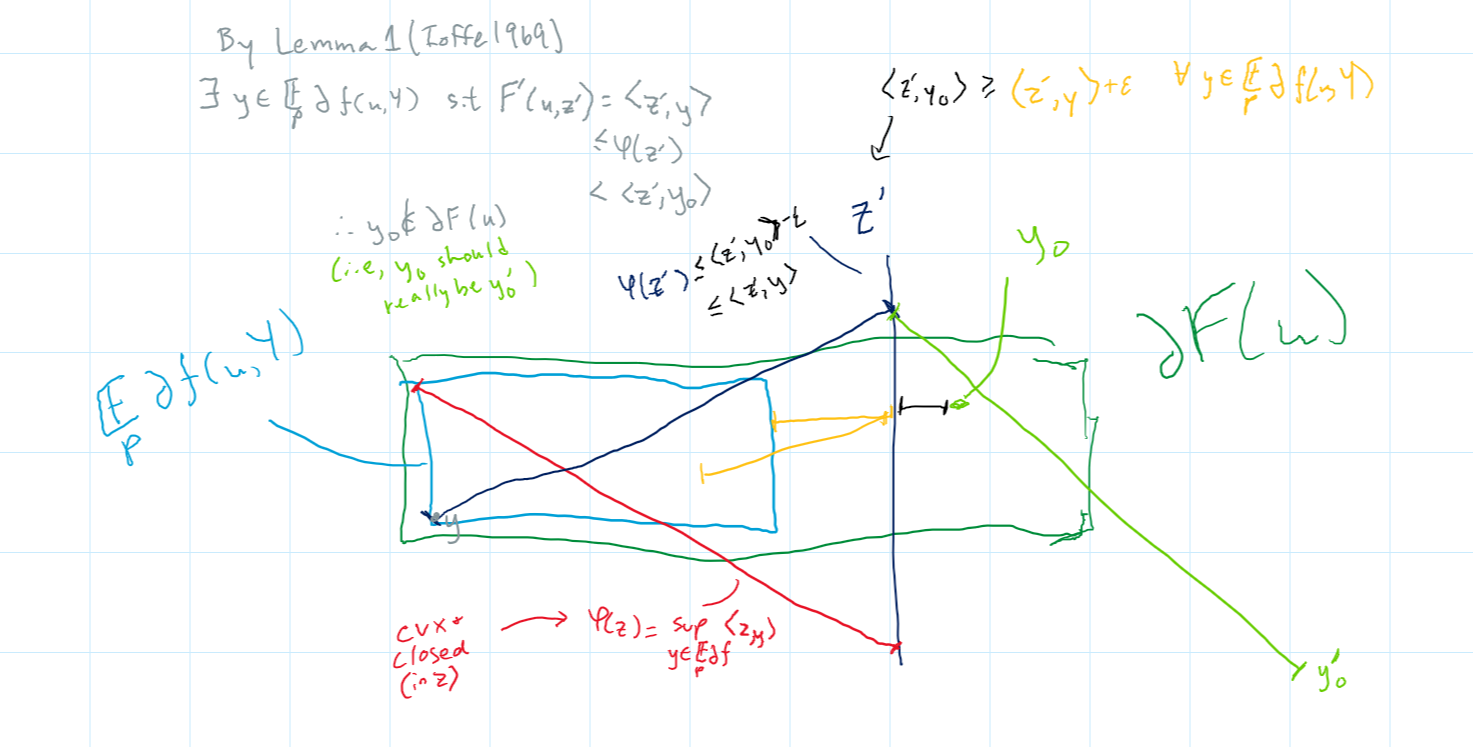
\includegraphics[width=0.7\linewidth]{tikz/ioffeproofpic}
	\caption[Picture understanding proof of Ioffe result]{}
	\label{fig:ioffeproofpic}
\end{figure}



\section{Result}
\begin{corollary}[\cite{rockafellar1982interchange}]
	Suppose $f$ is an $\A$-normal convex integrand such that $F(x) < \infty$ whenever $x \in \dom(f(\cdot,y))$ almost surely, where $F(x) = \E_p f(x,Y)$.
	
	Suppose moreover that there exists $x_0 \in \reals^d$ at which $F$ is finite and continuous, and that the multifunction $G: y \mapsto \cl(\dom(f(\cdot,y)))$ is almost surely constant.
	Then for all $x \in \reals^d$, we have $\E_p \partial f(x, \cdot) = \partial F(x)$.
\end{corollary}


\section{Examples}
We verify the satisfaction of the following three assumptions of the corollary:
\begin{enumerate}
	\item $f$ is a $\A$-normal convex integrand.
	\item $F(u) < \infty$ for $u \in \effdom(f(\cdot,y))$ almost surely (on $y$).
	\item There exists $x_0 \in \reals^d$ so that $\E_p f(x_0, Y)$ is (a) finite (b) continuous at $x_0$ and (c) $y \mapsto \cl \dom (f(\cdot, y))$ is almost surely constant.
\end{enumerate}
\subsection{$f(u,y) = |u|$.}

Since randomness is in $\Y$ and the loss function is not over $y$, so we know that $\E_p f(u,Y) = |u|$ regardless of $p$, therefore we can interchange expectation and subdifferentials no matter the distribution, but let's work through the conditions.

First, $H : y \mapsto \{(u,\alpha) : \alpha \geq |u| \}$ can be verified that the function is closed, convex-valued, and measurable.
Second, since $\E_p f(u,Y) = |u|$, $u \in \effdom(f)$ (almost surely) implies $u \in \reals$, and by substitution, we have $\E_p f(u,Y) = |u| < \infty$.
Third, Take $x_0 = 0$.  For all $p$, we have $\E_p f(x_0, Y) = 0$, and $f$ is continuous at $0$.

Therefore, the three conditions of the corollary are attained, and we confirm we can interchange expectation and subdifferentials.


\subsection{$f(u,y) = (u-y)^2$, $p$ is a Pareto distribution with $\alpha = 3/2$}
First, consider the pareto distrubtion with $t_a = 1$ and $\alpha = 3/2$ whose PDF is given 
\begin{equation*}
p(t) = \frac{3}{2t^{5/2}}, \,\,\, t > 1~,~
\end{equation*}
and is $0$ otherwise.

This distribution has mean $6$ and infinite variance.
Observe that this is Reviewer 6's ``counterexample'' they claimed did not work.
We want to understand which assumptions, if any, do not apply.

In particular, let's look at the second condition.
We want to verify that $\E_p (u-Y)^2 < \infty$ for all $x \in \effdom (f, \cdot, y)$ almost surely.
Take $u = 0$, and observe $f(0,y) = y^2$ is finite almost surely. 
However, $\E_p (u-Y)^2 = \E_p Y^2$, and since $p$ has infinite variance, this value is infinite as well.
Therefore, we do not satisfy the second condition of the corollary.


\subsection{$f(u,y) = (u-y)^2$, $p = \mathcal{N}(0,1)$}
Here's a softball... seemingly.
First, we can verify $y \mapsto \epi((u-y)^2)$ is closed, convex-valued, and measurable, as $f$ is convex in $u$ for constant $y$.

Next, consider $u \in \effdom(f(\cdot, y)$ almost surely iff $u \neq \pm \infty$.
That is, $(u - y)^2 = u^2 + y^2 - 2uy$ is finite for almost all $y$.
In this case, $F(u) = u^2 - [\E_p Y]^2 -2 u \E_p [Y]$.
Plugging in $p$, we have $F(u) = u^2$, which is finite as $u$ must be finite.

Finally, take $x_0 = 0$.
We can verify $F$ is finite and continuous at $x_0$.
Moreover, the function $y \mapsto \cl \dom f(0, y)$ is $\reals$ for all $y$, so the third condition holds.

Therefore, we can interchange subdifferentiation and expectation. 


\section{The bigger picture}
This matters so that we can generalize the proof of Theorem 2 to infinite outcome settings.

Essentially, we want to show that for convex losses, the level sets are unions of $d$-dimensional flats, which are loosely defined as the kernel space of a loss.

\hrule
From Zulip convo:

We can rewrite the statement "Every level set of a d-convex-elicitable property is the union of codim-d flats" as 
``$\Gamma$ is d-convex-elicitable $\implies \forall u, \exists \mathbb X \subseteq  (\cal Y \to\mathbb{R}^d)$  s.t.  $\Gamma_u = \bigcup_{X \in \mathbb{X}} \mathrm{ker} X \cap \,\,\Delta_{\mathcal{Y}}$''

The implication is weaker than showing that for all $u$ and $p \in \Gamma_u$, there is some $\bar X$ so that (a) $\bar X$ is $d$-dimensional and (b) $p \in \ker( \bar X)$.  ($\bar X$ dimension $d$ implies the flat, $Ker(\bar X)$, is codimension $d$.)

So now we assume $\Gamma$ is $d$-convex elicitable (by L), and want to show that such a $\bar X$ exists.

Fix u, and consider that $p \in \Gamma_u \iff \vec 0 \in \partial \mathbb{E}_p L(u,Y) = \{\E_p X(Y) : \forall y \in \mathcal{Y}, \, X(y) \in \partial L(u,y) \}$, where the first $\iff$ follows specifically since $\Gamma$ is convex elicitable.  
This implies $\exists \bar X$ in this set so that $\vec 0 = \E_p \bar X(Y)$.  
(well... if the conditions of the Corollary are satisfied.)  
Moreover, since $\E_p X(Y) \in \partial \mathbb{E}_p L(u,Y)$ and $L$ is $d$-dimensional, we have $\bar X$ is $d$-dimensional.

We can then (as before) construct the flat $ \ker(\bar X) \cap \Delta_{\mathcal{Y}}$.  
By construction, we have $p \in \ker(\bar X)$ and that the flat is at most codimension $d$.

\section{What's next?}
We want to understand the restrictions on (a) the loss and (b) on $\P$ that are made in order to apply this corollary (for all $p\in \P$).

Restrict to losses that are $\A$-normal convex integrands.
%... is this the same as identifiable functions?
%\jessie{Reminds me of~\cite[Theorem 5]{steinwart2014elicitation} and \cite[Theorem 2]{gneiting2011making}, but the former requires $\Gamma$ to be real valued and strictly locally non-constant...}


\jessie{Stronger assumption than necessary, but if we can show $L$ is continuous at $\Gamma(p)$, that covers condition 3}

\begin{theorem}[Theorem 2]
	Let a property $\gamma : \P \toto \R$ be given, and let $p \in \P$, and $r \in \gamma(p)$.
	Let $L : \reals^d \times \Y \to \reals$ be a convex loss\footnote{must be a $\A$ convex normal integrand} such that such that $\E_p L(\cdot,Y)$ is finite for all $u \in \reals^d$.
	If $L$ indirectly elicits $\gamma$, there is a flat $F$ with $p \in F \cap \P \subseteq \gamma_r$ with $\codim(F) \leq d$.
\end{theorem}
\begin{proof}
	Consider the probability space $(\Y, \A, p)$, where $p \in \P$, and let $\Gamma := \prop{L}$.
	Moreover, suppose $(L, \psi)$ indirectly elicits $\gamma$.
	By definition of properties, there is some $u \in \Gamma(p)$.
	
	We first construct the flat $F$ and show $F \cap \P \subseteq \Gamma_u$, which implies $F \cap \P \subseteq \gamma_r$ by indirect elicitation \jessie{though this needs more detail since we don't necessarily have $u = \psi(r)$.}. 
	
	As $L$ is convex and elicits $\Gamma$, we have $u \in \Gamma(p) \iff \vec 0 \in \partial \E_p L(u,Y)$.
	Since, for each $p \in \P$ by Lemma~\ref{lem:conditions-sat}, $L$ satisfies the assumptions of~\cite[Corollary 1]{rockafellar1982interchange}, we also have $\vec 0 \in \partial \E_p L(u,Y) \iff \vec 0 \in \E_p \partial L(u,Y) := \cl(\{\int \nu(y) p(dy) : \nu \in \L^1_d(\A), \nu(y) \in \partial L(u,Y)\,\, a.s.\})$.
	As $\vec 0$ is in the expectation of the subgradient, such a $\nu$ exists in the closure of this set.
	We now take $F := \ker(\nu) \cap \P$.
	
	By construction we have $\vec 0 = \E_p \nu(Y)$, meaning $p \in \ker(\nu) \cap \P = F$.
	Moreover, we have that $\codim(F) = \dim(\P \setminus F) \leq d$ since \jessie{rationale.}
\end{proof}

\begin{lemma}\label{lem:conditions-sat}
	For convex $L : \reals^d \times \Y \to \reals$ eliciting the nonempty property $\Gamma:\P\toto\R$, if $\P$ is a set such that $\E_p L(u,Y) < \infty$ for all $u \in \reals^d$ and $p \in \P$, then the conditions of \cite[Corollary 1]{rockafellar1982interchange} are satisfied.
\end{lemma}
\begin{proof}
	First, we enumerate the conditions of \cite[Corollary 1]{rockafellar1982interchange}.\begin{enumerate}
		\item $L$ is a $\A$-normal convex integrand.
		\item $\E_p L(u,Y) < \infty$ for $u \in \effdom(L(\cdot,y))$ almost surely (on $y$).
		\item There exists $x_0 \in \reals^d$ so that $\E_p f(x_0, Y)$ is (a) finite and (b) continuous at $x_0$
		\item $y \mapsto \cl \dom (f(\cdot, y))$ is almost surely constant.
	\end{enumerate}


As we constrain $L$ to be real-valued, the effective domain and domain are equal, and assumed to be $\reals^d$.
The first condition follows by assumption that $L$ is $\B(\reals^d) \otimes \A$-measurable and lower semi-continuous.
Therefore, the second condition is satisfied when $\E_p L(u,Y)$ is finite for all $u \in \reals^d$, by assumption on $\P$.
Third, for each $p$, take $x_0 \in \Gamma(p)$.
As $L$ is finite, we know that $\E_p L(\Gamma(p), Y)$ is finite.
Moreover, $\E_p L(\cdot, Y)$ is continuous at $x_0$ by convexity of $L$ in its first argument and the assumption that $L(u,y)$ is finite for all $u,y$. \jessie{Don't think this is accurate}
The final condition follows by assumption on $L$.
\end{proof}

\bibliographystyle{ieeetr}
\bibliography{diss,extra}

\end{document}